
\newcommand{\JvolveTimeLine}[5]{
\begin{center}
\begin{tikzpicture}[auto]
  \tikzstyle{block}=[
    font=\tiny,
    rectangle,
    draw=structure.fg,
    thick,
    text width=1.2cm,
    text badly centered,
    rounded corners,
    minimum height=2em,
  ]
  \tikzstyle{current}=[fill=structure.fg!20, ]
  \tikzstyle{line}=[draw, thick, -latex',]
  \tikzstyle{every path}=[line]
  \matrix [column sep=5mm,row sep=7mm,ampersand replacement=\&] {
    \node [block,#1] (0) {\hyperlink{offline}{Offline tool}};          \&
    \node [block,#2] (1) {\hyperlink{suspend}{Suspend application}};   \&
    \node [block,#3] (2) {\hyperlink{classload}{Load new classes}};    \&
    \node [block,#4] (3) {\hyperlink{transform}{Transform objects}};   \&
    \node [block,#5] (4) {Resume application};                         \\
  };
  \path (0) -- (1);
  \path (1) -- (2);
  \path (2) -- (3);
  \path (3) -- (4);
\end{tikzpicture}
\end{center}
}


\begin{frame}[t,fragile]{Update process}%{A Sub-title is optional}
% \JvolveTimeLine{}{current}{}{current}{}
\begin{itemize}
\item Offline Update Preparation Tool
\item \DSU{} VM
  \begin{itemize}
  \item Reach a DSU safe point
  \item Install new classes
  \item Update state
  \item Resume execution
  \end{itemize}
\end{itemize}
\end{frame}

\section{Update Timing and Safety}
% \ShowTOC

% \begin{frame}{Check for update safety}%{A Sub-title is optional}
% \vspace*{-3mm}%
% \begin{center}%
% 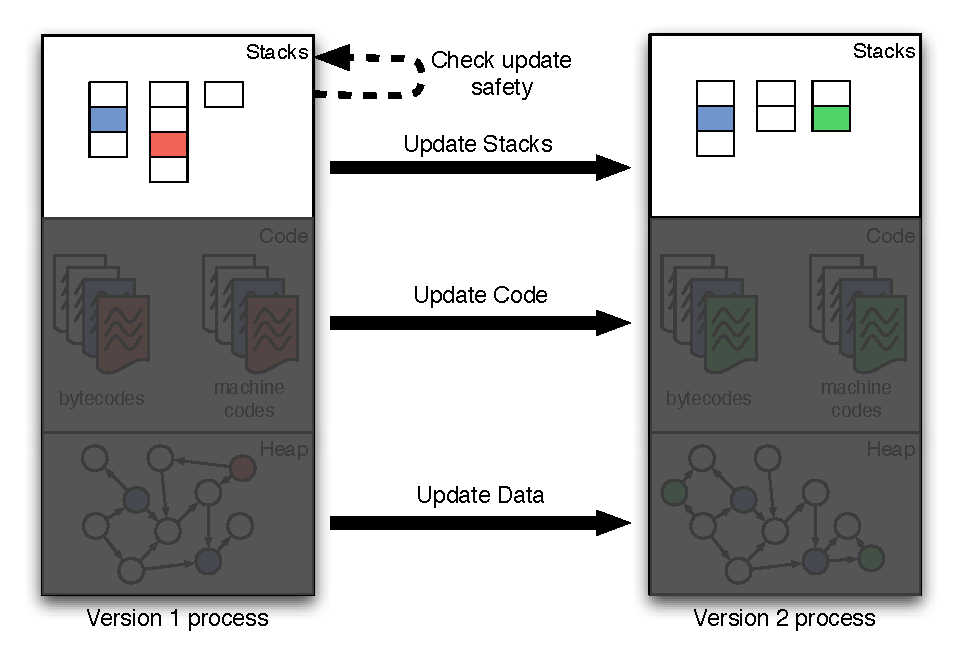
\includegraphics[scale=0.73]{images/process-state/both-process-state-highlight-stack}%
% \end{center}%
% \end{frame}

\begin{frame}[t,label=suspend]{Safe point for the update}%{A Sub-title is optional}
\begin{textblock*}{0mm}[0,0](90mm,11mm)%
\only<1>{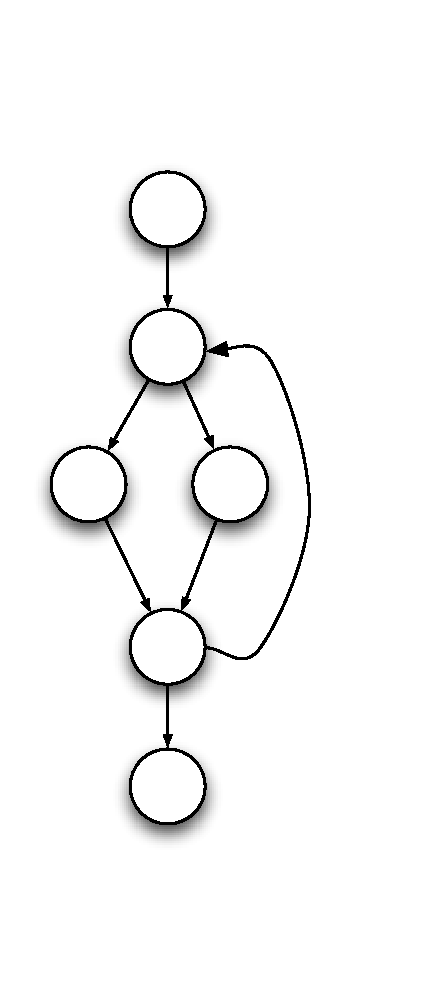
\includegraphics[scale=0.475]{images/yieldpoint/cfg}}%
\only<2->{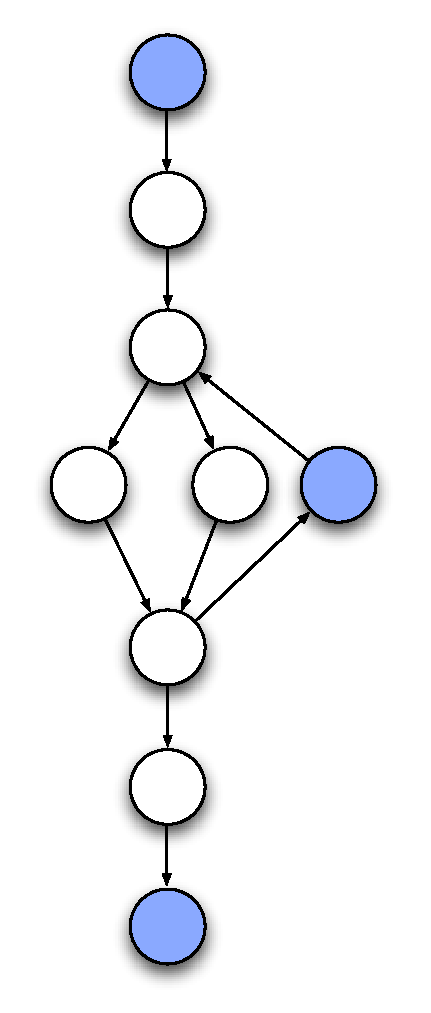
\includegraphics[scale=0.475]{images/yieldpoint/cfg-with-yieldpoint}}%
\end{textblock*}%
\begin{itemize}%
\item Updates happen at ``safe points''
\item Safe points are VM yield points, \\
      and restrict what methods can be on stack
\item<3> Extend the thread scheduler to \\
      suspend all application threads
\item<3> If any stack has a restricted method, \\
      delay the update
\end{itemize}%
\end{frame}

\begin{frame}{Restrict changed methods (activeness safety)}%{A Sub-title is optional}
\begin{itemize}
\item Update happens atomically
\item Only old code runs before update, only new after update
\item Do not allow changed methods to be active on stack
\item Guarantees type safety
\item Old and new version methods are independently type-safe
\end{itemize}
\begin{center}
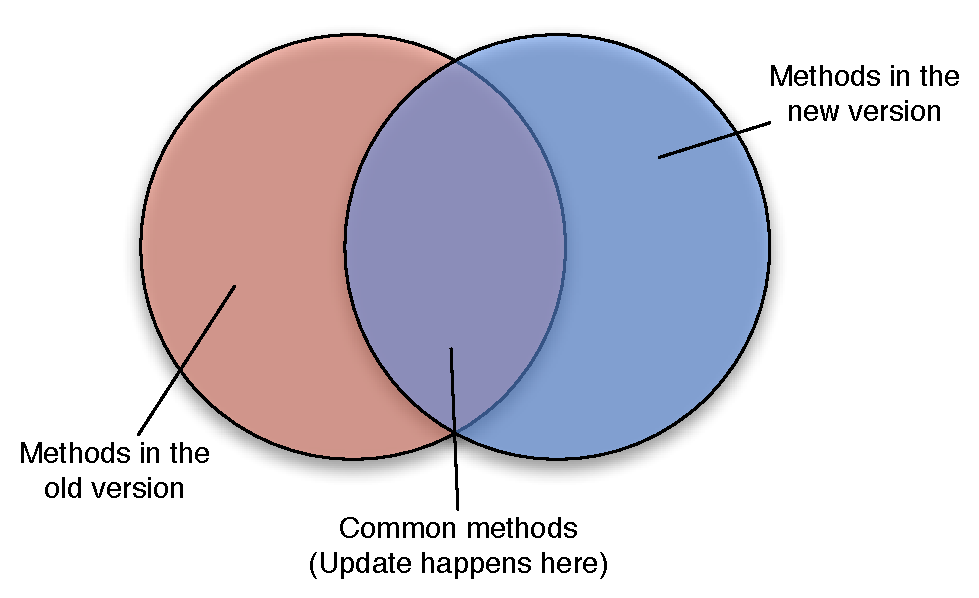
\includegraphics[scale=0.38]{images/activeness-venn-diagram}
\end{center}
\end{frame}

\begin{frame}[t,fragile]{Restricted methods}%{A Sub-title is optional}
\begin{enumerate}[(1)]
\item Methods changed by the update
\item Methods identified by the user as unsafe based on semantic
information about the application
\begin{block}{}
Install return barriers that trigger DSU upon unsafe method's return
\end{block}
\vspace{2ex}
\item<2> Methods whose bytecode is unchanged, but compiled representation is
      changed by the update
  \begin{itemize}
  \item Offsets of fields and methods hard-coded in machine code
  \item Inlined callees may have changed
  \end{itemize}
\begin{block}{}
Utilize on-stack replacement to recompile base-compiled methods
\end{block}
\end{enumerate}
\end{frame}

% \begin{frame}{Handling restricted methods}%{A Sub-title is optional}
% \vspace*{-2mm}%
% \begin{center}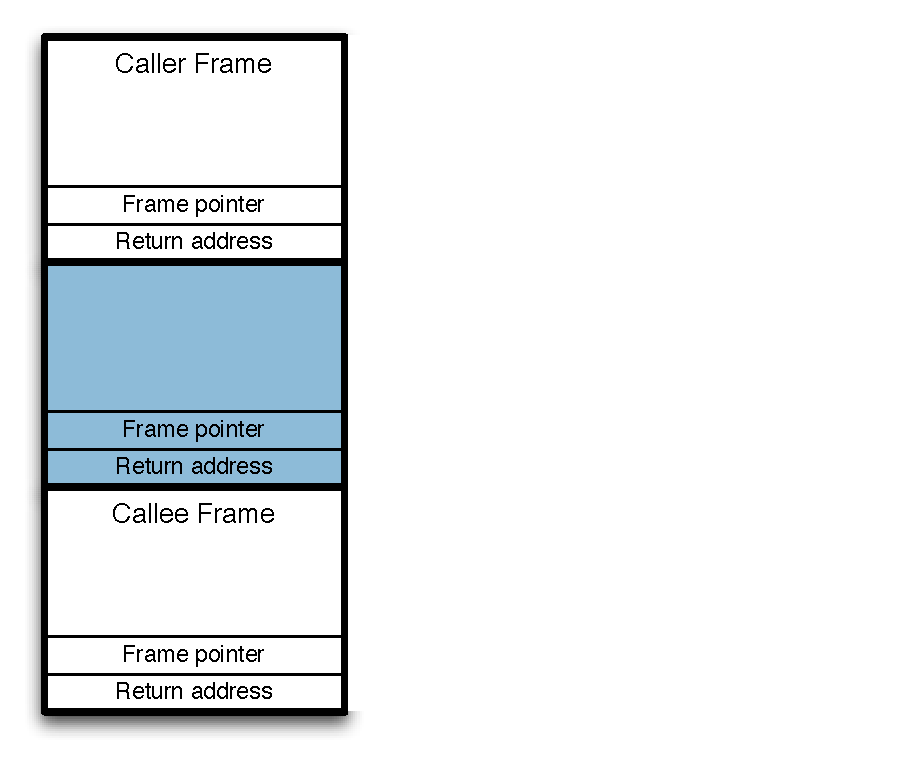
\includegraphics[scale=0.62]{images/stack-smash/stack-frames-overview}\end{center}
% \end{frame}
% 
% \begin{frame}{Installing return barrier for DSU}%{A Sub-title is optional}
% \vspace*{-2mm}%
% \begin{center}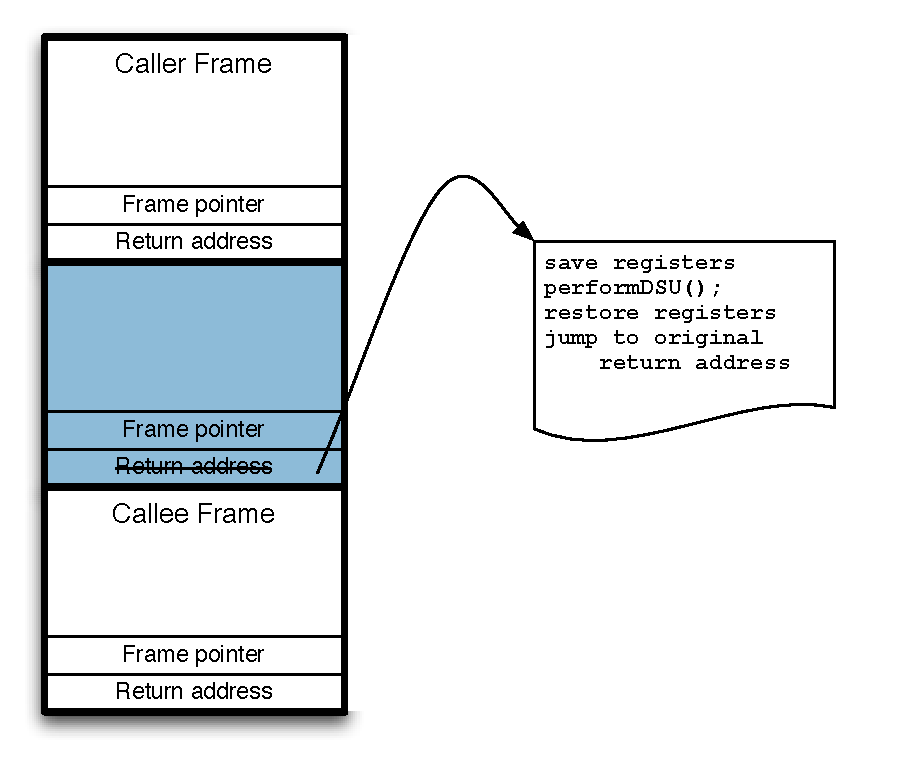
\includegraphics[scale=0.62]{images/stack-smash/return-barrier-overview}\end{center}
% \end{frame}
% 
% \begin{frame}{Performing On-stack replacement}%{A Sub-title is optional}
% \vspace*{-2mm}%
% \begin{center}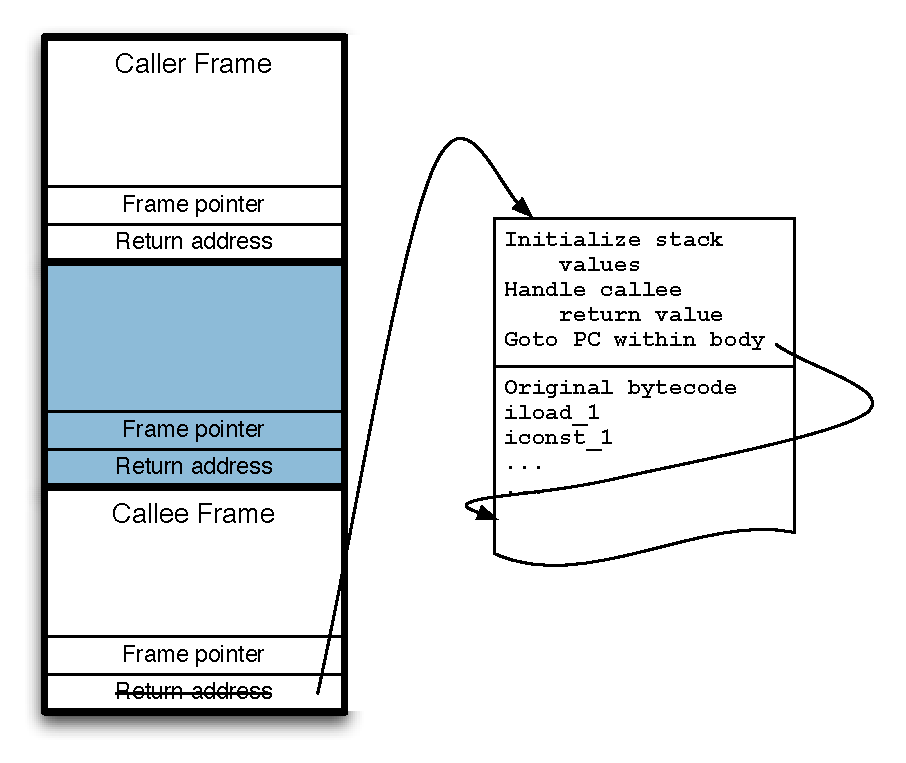
\includegraphics[scale=0.62]{images/stack-smash/osr-overview}\end{center}
% \end{frame}

\begin{frame}{Reaching a safe point}%{A Sub-title is optional}
\hspace*{-3mm}
\begin{center}
\scalebox{0.44}{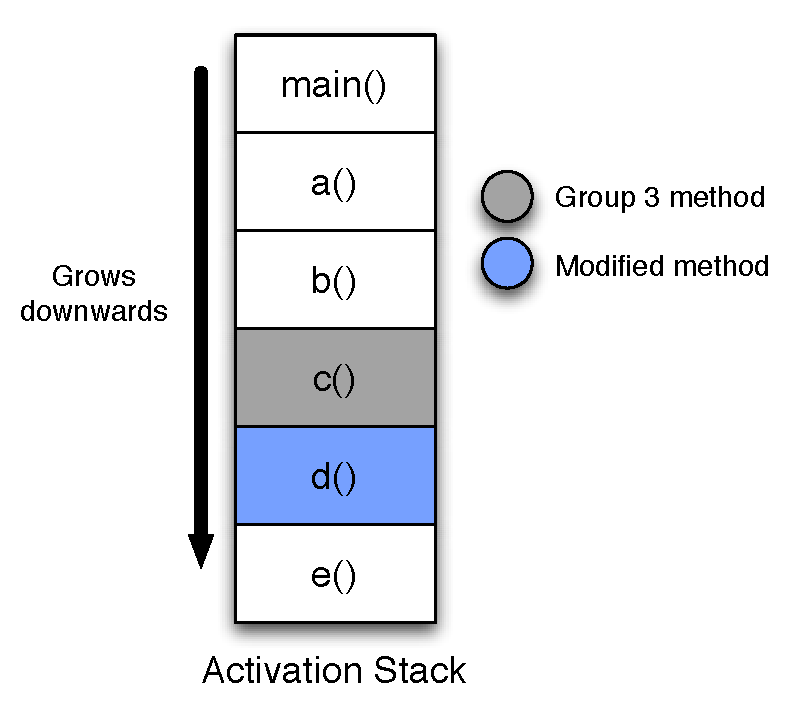
\includegraphics{images/safe-point-call-graph/simple-activation-stack}}
\begin{block}{}
Install a return barrier for d(). Wait till it returns. On-stack replace
new machine code for c().
\end{block}
\end{center}
\end{frame}
